\input{preamble.tex}

\title{\huge{Assignment 1}}
\author{\LARGE{Thobias Høivik}}
\date{}

\begin{document}
\maketitle

\newpage
Jeg pleier generellt sett å gjøre matematikk 
på Engelsk. Jeg skal prøve å 
følge ordboken, men viss det 
er noen litt feil begrep beklager 
jeg dette. 

\begin{prob*}[1]
    Let $M$ be an $R$-module of finite length, i.e. 
    an $R$-module that admits a composition of series. 
    Show that: 
    \begin{enumerate}[label=\alph*)]
        \item If $N < M$ is a proper submodule of $M$, then
            $l(N) < l(M)$.  
        \item Every composition series for $M$ has length 
            $l(M)$. 
        \item Every chain $0 = M_0 \subsetneq M_1 \subsetneq 
            M_2 \subsetneq \cdots \subsetneq M_n = M$ of 
            submodules of $M$ can be refined to a composition 
            of series for $M$. 
    \end{enumerate}
\end{prob*}
\begin{proof}[Bevis for (a)]
    La $N < M$ være en ekte undermodul av $M$. 
    Siden $M$ har endelig lengde, så har vi at 
    vi kan finne en komposisjon 
    \[
        0 = M_0 < M_1 < \cdots < M_n = M. 
    \]
    Siden $N \subseteq M$, har vi da at 
    \[
        N \cap M = N, 
    \]
    så 
    \[
        0 = N \cap M_0 \subseteq N \cap M_1 \subseteq \cdots 
        \subseteq N \cap M_n = N. 
    \]
    Siden kjeden for $M$ utgjør en komposisjonsserie 
    har vi at 
    \[
        \frac{M_i}{M_{i-1}}
    \]
    er simpel for alle $i \in [m] $. 

    Vi vil argumentere 
    ved å bruke isomorfi teoremet. 

    La $\varphi : N \cap M_i \to \frac{M_i}{M_{i-1}}$ være 
    \[
        \varphi(n) = n + M_{i-1}. 
    \]
    Da har vi at 
    \begin{align*}
        \varphi(n + m) 
        &= (n + m) + M_{i-1} \\ 
        &= n + M_{i-1} + M_{i-1} \\ 
        &= \varphi(n) + \varphi(m). 
    \end{align*}
    Deretter, for $r \in R$, 
    \begin{align*}
        \varphi(rn) 
        &= (rn) + M_{i-1} \\ 
        &= r (n + M_{i-1}), 
    \end{align*}
    så $\varphi$ utgjør en $R$-modul 
    homomorfi. 

    Vi har $x + M_i = 0$ modulo $M_{i-1}$ viss og bare 
    viss 
    \[
        x \in M_{i-1}
    \]
    så 
    \[
        \ker \varphi = (N\cap M_i) \cap M_{i-1} 
        = N \cap M_{i-1}.
    \]

    $\operatorname{Im}(\varphi) \subseteq \frac{M_i}{M_{i-}}$ 
    en undermodul, så siden $\frac{M_i}{M_{i-1}}$ er 
    simpel er bildemengden til $\varphi$ triviell eller 
    $\frac{M_i}{M_{i-1}}$. 

    Dermed har vi at 
    \[
        \frac{N \cap M_i}{M_{i-1}} 
        \cong 
        \operatorname{Im}(\varphi) 
        \begin{cases}
            0, \\ 
            M_{i}/M_{i-1}
        \end{cases}.
    \]
    
    Med dette har vi $l(N) \leq l(M)$. 
    
    Siden $M_n \not\subseteq N$ har vi at 
    \[
        \{i \in [n] \bigm| M_i \not\subseteq N\} \neq \emptyset.  
    \]
    For den minste $j$ i denne mengden har vi at 
    \[
        M_{j-1} \subseteq N 
    \]
    og at 
    \[
        M_j \not\subseteq N. 
    \]
    Vi sletter alle $M_j$ der dette er tilfellet og 
    sitter fortsatt igjen med en komposisjonsserie for 
    $N$ så $l(N) < l(M)$.
\end{proof}

\begin{proof}[Bevis av (b)]
    Vi vil bevise ved induksjon på $l(M)$ at alle 
    komposisjonsserier for $M$ har samme lengde.

    Hvis $l(M)=0$, så er $M=0$, og påstanden er triviell.

    Anta nå at påstanden holder for alle moduler med lengde 
    mindre enn $l(M)$.

    La
    \[
        0=M_0\subsetneq M_1\subsetneq\cdots
        \subsetneq M_{n-1}\subsetneq M_n=M
    \]
    og
    \[
        0=N_0\subsetneq N_1\subsetneq\cdots
        \subsetneq N_{m-1}\subsetneq N_m=M
    \]
    være to komposisjonsserier for $M$.

    Siden
    \[
        M/M_{n-1}
        \qquad\text{og}\qquad
        M/N_{m-1}
    \]
    er simple, er $M_{n-1}$ og $N_{m-1}$ maksimale
    undermoduler av $M$.

    Hvis
    \[
        M_{n-1}=N_{m-1},
    \]
    så er de to trunkerte seriene
    \[
        0\subsetneq M_1\subsetneq\cdots\subsetneq M_{n-1}
    \]
    og
    \[
        0\subsetneq N_1\subsetneq\cdots\subsetneq N_{m-1}
    \]
    komposisjonsserier for samme modul $M_{n-1}$.
    Siden
    \[
        l(M_{n-1})<l(M),
    \]
    gir induksjonshypotesen at
    \[
        n-1=m-1,
    \]
    og dermed $n=m$.

    Anta derfor at
    \[
        M_{n-1}\neq N_{m-1}.
    \]
    Siden $M_{n-1}$ er maksimal og
    $N_{m-1}\not\subseteq M_{n-1}$, får vi
    \[
        M_{n-1}+N_{m-1}=M.
    \]

    Sett
    \[
        K=M_{n-1}\cap N_{m-1}.
    \]
    Ved andre isomorfiteorem har vi
    \[
        \frac{M_{n-1}}{K}
        \cong
        \frac{M_{n-1}+N_{m-1}}{N_{m-1}}
        =
        \frac{M}{N_{m-1}},
    \]
    og tilsvarende
    \[
        \frac{N_{m-1}}{K}
        \cong
        \frac{M}{M_{n-1}}.
    \]
    Begge kvotientene er simple.

    Siden $K$ er en ekte undermodul av $M$, har vi
    \[
        l(K)<l(M).
    \]
    La
    \[
        0=K_0\subsetneq K_1\subsetneq\cdots
        \subsetneq K_r=K
    \]
    være en komposisjonsserie for $K$.

    Siden $M_{n-1}/K$ er simpel, får vi en
    komposisjonsserie
    \[
        0=K_0\subsetneq\cdots\subsetneq K_r=K
        \subsetneq M_{n-1}
    \]
    for $M_{n-1}$.
    Ved induksjonshypotesen må denne ha samme lengde som
    \[
        0=M_0\subsetneq\cdots\subsetneq M_{n-1}.
    \]
    Dermed
    \[
        n-1=r+1.
    \]

    På samme måte får vi
    \[
        m-1=r+1.
    \]
    Følgelig
    \[
        n=m.
    \]

    Dermed har alle komposisjonsserier for $M$ samme lengde,
    nemlig $l(M)$.
\end{proof}
\begin{proof}[Bevis av (c)]
    Vi vil bevis at viss vi har en vilkårlig kjede 
    \[
        0 = M_0 \subsetneq M_1 \subsetneq \cdots 
        \subsetneq M_n = M 
    \]
    så kan vi rafinere dette til en komposisjons serie 
    for $M$, altså at 
    \[
        M_i/M_{i-1}
    \]
    er simpel. 

    Viss vi har at 
    \[
        M_i/M_{i-1}
    \]
    ikke er simpel, må det finnes en 
    maksimal undermodul $N$ 
    \[
        M_{i-1} \subsetneq N \subsetneq M_i 
    \]
    siden $M_i$ ikke er simpel. 
    Vi kan gjøre dette for alle $i$ hvor $M_i/M_{i-1}$
    ikke er simpel. Det som gjennstår er at 
    vi må vise at gjenntatte applikasjoner av denne prosedyren 
    på den nye kjeden vi får må til slutt stoppe. 
    Ved hver $M_i$ har vi at $M_i$ har endelig lengde 
    $\ell(M_i)$ og at 
    \[
        \ell(M_{i-1}) < \ell(M_i) 
    \]
    og 
    \[
        \ell(M_i) \leq \ell(M) \neq \infty 
    \]
    så hver $M_i$ kan ikke ha mer enn $\ell(M)$ 
    ekte undermoduler så prosedyren vil produsere 
    en endelig kjede hvor kvotienten av $M_i$ med $M_{i-1}$
    er simpel. 
\end{proof}

\begin{prob*}[2]
    \medskip 
    \   
    
    \begin{enumerate}[label=\alph*)]
        \item Find a composition series for 
            $\mathbb Z_{60}$. 
        \item Let $k$ be a field, and find a composition 
        series for the $k[x,y]$-module $M = k[x,y]/(x^2,xy,y^3)$.
        \item For $M = \mathbb Z_{126}$, give two distinct 
        series 
        \[
            (0) = M_0 \subsetneq M_1 \subsetneq M_2 \subsetneq M_3 = M
        \] 
        and show how each of them may be extended to a composition series.
    \end{enumerate}
\end{prob*}
\begin{proof}[Løsning til (a)]
    En maksimal undermodule for $\mathbb Z_{60}$ er 
    \[
        \langle \overline 2 \rangle \cong \mathbb Z_{30}. 
    \]
    Deretter er $\mathbb Z_{15} \cong 
    \langle \overline 4 \rangle$ en maksimal undermodul 
    av $\mathbb Z_{30}$. Deretter har vi $\mathbb Z_5 < 
    \mathbb Z_{15}$ som har kun den trivielle undermodulen 
    $0$. 
    Vi får da en komposisjonsserie der hvert ledd 
    er lik, eller isomorf til 
    \[
        0 < \mathbb Z_5 < \mathbb Z_{15} < \mathbb Z_{30}
        < \mathbb Z_{60}.
    \]
    Den faktiske serien blir da 
    \[
        0 < \langle \overline{12} \rangle 
        < \langle \overline 4 \rangle 
        < \langle \overline 2 \rangle 
        < \mathbb Z_{60}. 
    \]
\end{proof}

\begin{proof}[Løsning for (b)]
    Som et $k$-vektorrom har vi 
    \[
        \frac{k[x,y]}{(x^2, xy, y^3)} 
        = \operatorname{span}_k\{\overline 1, \overline x, 
        \overline y, \overline{y^2}\}
    \]
    så lengden (dimensjonen i konteksten av vektorrom) 
    er $4$. 

    $k \overline{y^2}$er en undermodul siden 
    $x\overline{y^2} = \overline{y(xy)} = 0$,
    og $y\overline{y^2} = \overline{y^3} = 0$. 

    Vi fortsetter deretter med $k\bar y + k\overline{y^2}$. 
    Der har vi $x\bar y = \overline{xy} = 0$, 
    $y\bar y = \overline{y^2} = 0$, 
    $x\overline{y^2} = 0$, $y\overline{y^2} = 0$. 

    Til slutt har vi modulen 
    $k\bar x + k\bar y + k \overline{y^2}$. 

    \[
        0
        <
        M_1 := k\overline{y^2}
        <
        M_2 := k\bar y+k\overline{y^2}
        <
        M_3 := k\bar x+k\bar y+k\overline{y^2}
        <
        M.
    \]

    Vi har $M_1/0$ generert av $\overline{y^2}$, 
    $M_2/M_1$ generert av $\bar y$, $M_3/M_2$ generert av 
    $\bar x$ og $M/M_3$ generert av $1$, så 
    dette er en komposisjonsserie. 
\end{proof}

\begin{proof}[Løsning til (c)]
    Vi har $\langle \overline 2 \rangle \cong 
    \mathbb Z_{63}< \mathbb Z_{126}$ 
    og $\langle \overline 3 \rangle \cong 
    \mathbb Z_{42} < \mathbb Z_{126}$ er maksimale undermoduler. 

        Deretter har vi $\langle \overline 6 \rangle 
        \cong \mathbb Z_{21} < \langle \overline 2 \rangle$ 
        er maksimal og 
        $\langle \overline 6 \rangle \cong 
        \mathbb Z_{21} < \langle \overline 3 
        \rangle $ 
        er maksimal. 

        Så vi får de to kjedene 
        \[
            0 \subsetneq \langle \overline 6 \rangle 
            \subsetneq \langle \overline 2 \rangle 
            \subsetneq \mathbb Z_{126},
        \]
        og 
        \[
            0 \subsetneq \langle \overline 6 \rangle 
            \subsetneq \langle \overline 3 \rangle 
            \subsetneq \mathbb Z_{126}.
        \]
        $\langle \overline 6 \rangle / 0 = \langle \overline 6 
        \rangle \cong \mathbb Z_{21}$ er ikke simpel.  

        En maksimal undermodul av den er $\langle \overline{18} 
        \rangle \cong \mathbb Z_{7}$ som er simpel. 

        Så de to kjedene kan rafineres 
        til komposisjonsserier 
        begge med lengde $4$. 
\end{proof}

\begin{figure}[htbp]
    \centering
    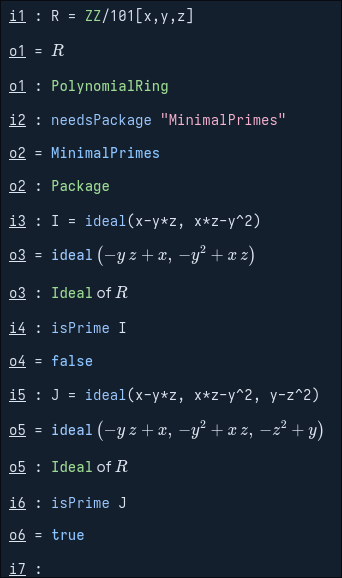
\includegraphics[width=0.8\textwidth]{./macaulay-printout.png}
    \caption{Problem 3.1 \& 3.2}
    \label{fig:macaulay}
\end{figure}

\newpage 

\begin{proof}[Løsning (a,b,c)]
    Vi har $I = (x-yz, xz-y^2)$. 
    For å finne $V(I)$ trenger vi alle 
    \[
        (x,y,z) \in k^3
    \]
    hvor $x-yz = 0$ og $xz-y^2 = 0$. 

    Fra første ligning: 
    \[
        x=yz. 
    \]
    Dette lar oss fjerne $x$. Substituter inn 
    i denne andre ligningen: 
    \[
        xz - y^2 = 0.
    \]
    Siden $x = yz$, 
    \[
        (yz)z - y^2 = 0,
    \]
    så 
    \[
        y(z^2 - y) = 0. 
    \]
    $k$ er en kropp så $y = 0$ eller $z^2 = y$. 

    Case 1: 

    Siden 
    \[
        x = yz, 
    \]
    har vi 
    \[
        x = 0. 
    \]
    Men $z$ kan være hva som helst. 
    Dermed får vi hele linjen: 
    \[
        (0,0,t), \ t \in k. 
    \]

    Case 2: 

    Viss $y = z^2$, 
    har vi (siden $x=yz$) 
    \[
        x = z^3. 
    \]
    Så vi får en parameterisert kurve 
    \[
        (t^3, t^2, t), \ t \in k. 
    \]
    Sammen: 
    \[
        V(I) = \{(0,0,t) \bigm| t \in k\} 
        \cup \{(t^3,t^2,t) \bigm| t \in k\}. 
    \]

    Nå ser vi på $V(J)$. 
    \[
        J=(x-yz,\;xz-y^2,\;y-z^2).
    \]
    Igjen, $x = yz$ og vi vet 
    $y = z^2$. 
    Dermed har vi 
    \[
        x = yz = z^3. 
    \]
    Så alle punkt har formen 
    \[
        (x,y,z) = (t^3,t^2,t). 
    \]
    $xz-y^2 = 0$ er da automatisk tilfredsstilt siden 
    \[
        xz - y^2 = (t^3)t - (t^2)^2 = t^4 - t^4 = 0. 
    \]

    Ligningen i idealet som ikke var prim 
    splitter til to uavhengige muligheter, mens 
    for $J$ er det en enkelt parameterisert kurve som 
    tilfredsstiller ligningene vi får av $J$. 
\end{proof}


\end{document}
